%------------------------------------------------------------
% Proyecto 2 — Algoritmos de Búsqueda en Laberintos
% Inteligencia Artificial 2026
%------------------------------------------------------------
\documentclass[12pt,a4paper]{article}

\usepackage[utf8]{inputenc}
\usepackage[T1]{fontenc}
\usepackage[spanish]{babel}
\usepackage{geometry}
\geometry{margin=2.5cm}

\usepackage{graphicx}
\usepackage{float}
\usepackage{booktabs}
\usepackage{array}
\usepackage{amsmath}
\usepackage{amsfonts}
\usepackage{hyperref}
\usepackage{xcolor}
\usepackage{caption}
\usepackage{subcaption}
\usepackage{enumitem}
\usepackage{parskip}

\hypersetup{colorlinks=true, linkcolor=blue, urlcolor=blue}

%------------------------------------------------------------
\title{%
  \textbf{Proyecto 2: Algoritmos de Búsqueda en Laberintos}\\[4pt]
  \large Inteligencia Artificial --- 2026
}
\author{
  Dilary Cruz (231010) \and
  June Herrera (231038) \and
  Andrés Mazariegos (21749)
}
\date{11 de mayo de 2026}

\begin{document}
\maketitle
\tableofcontents
\newpage

%============================================================
\section{Introducción}
%============================================================

Este proyecto tiene como objetivo comparar el desempeño de cuatro
algoritmos clásicos de búsqueda en grafos --- BFS, DFS, UCS y A* ---
para resolver laberintos generados aleatoriamente.

La experimentación se divide en tres problemas:
\begin{enumerate}
  \item Generación aleatoria de laberintos mediante los algoritmos de
        Kruskal y Prim.
  \item Resolución de un laberinto $60\times80$ con el algoritmo A*,
        incluyendo visualización del área explorada y del camino
        encontrado.
  \item Comparación cuantitativa de los cuatro algoritmos sobre $K=25$
        escenarios con laberintos de $45\times55$.
\end{enumerate}

Todos los experimentos fueron implementados en Python 3.13 usando
NumPy para la representación matricial, Matplotlib para las
visualizaciones y Pandas para el análisis de resultados.

%============================================================
\section{Algoritmos de Generación de Laberintos}
%============================================================

Un \textbf{laberinto perfecto} es un grafo conexo acíclico (árbol)
sobre una retícula $M\times N$: no contiene ciclos y desde cualquier
celda existe exactamente un camino hacia cualquier otra. Generarlo es
equivalente a encontrar un árbol de expansión del grafo reticular, lo
que explica el uso de algoritmos de MST.

\subsection{Representación interna}

Cada celda $(r,c)$ almacena un bitmask de 4 bits que indica qué muros
están \emph{abiertos}:
\[
  \text{bit}_0 = \text{Norte},\quad
  \text{bit}_1 = \text{Sur},\quad
  \text{bit}_2 = \text{Este},\quad
  \text{bit}_3 = \text{Oeste}.
\]
Estado inicial: todos los bits en 0 (todos los muros cerrados).
Eliminar la pared entre dos celdas adyacentes activa el bit
correspondiente en \emph{ambas} celdas. Esta representación ocupa
solo 1 byte por celda y permite consultar y modificar cualquier muro
en $O(1)$.

Para la visualización se utiliza una imagen de píxeles de tamaño
$(2M+1)\times(2N+1)$, donde las celdas ocupan las posiciones de
índices impares y las paredes las de índices pares, permitiendo un
renderizado en tiempo constante con una sola llamada a \texttt{imshow}.

\subsection{Kruskal aleatorizado}

\paragraph{Idea.}
Se listan todas las aristas potenciales del grafo reticular (pares de
celdas adyacentes), se \emph{mezclan} aleatoriamente y se procesan en
orden. Una arista se acepta ---y el muro correspondiente se elimina---
si y solo si une dos componentes distintas, determinado mediante una
estructura Union-Find. El proceso termina cuando el árbol abarca todas
las celdas.

\paragraph{Pseudocódigo.}
\begin{enumerate}
  \item $E \leftarrow$ todas las aristas de la grilla;\;
        $\texttt{shuffle}(E)$ con semilla fija.
  \item Inicializar Union-Find con $M\cdot N$ nodos.
  \item Para cada arista $(u,v)\in E$:\\
        \quad Si $\texttt{find}(u)\neq\texttt{find}(v)$:
        eliminar muro entre $u$ y $v$;\; $\texttt{union}(u,v)$.
\end{enumerate}

\paragraph{Complejidad.}
$O(E\,\alpha(V))$, donde $E = 2MN - M - N$ y $\alpha$ es la función
inversa de Ackermann (prácticamente constante). El Union-Find usa
unión por rango con compresión de caminos.

\paragraph{Característica visual.}
Kruskal construye el laberinto de forma \textbf{global}: abre pasajes
en regiones aparentemente desconectadas de forma simultánea, produciendo
un patrón uniforme y sin preferencia por ninguna zona del grid.

\subsection{Prim aleatorizado}

\paragraph{Idea.}
Se parte de una celda inicial aleatoria, marcada como visitada. Se
mantiene una lista de \emph{fronteras}: muros candidatos entre una
celda visitada y una no visitada. En cada paso se selecciona una
frontera al azar; si el vecino aún no fue visitado, se elimina el muro,
se marca el vecino como visitado y se añaden sus fronteras a la lista.

\paragraph{Pseudocódigo.}
\begin{enumerate}
  \item Marcar celda de inicio;\; agregar sus muros a $F$.
  \item Mientras $F \neq \emptyset$:\\
        \quad Seleccionar $(u,v)\in F$ aleatoriamente.\\
        \quad Si $v$ no visitado: eliminar muro;\; marcar $v$;\;
        agregar fronteras de $v$ a $F$.\\
        \quad Eliminar $(u,v)$ de $F$.
\end{enumerate}

\paragraph{Complejidad.}
$O(E\log E)$ en el peor caso por las operaciones sobre la lista de
fronteras.

\paragraph{Característica visual.}
Prim crece \textbf{localmente} desde un punto de origen, produciendo
laberintos con una estructura radial más pronunciada, pasajes más
largos cerca del origen y ramificaciones densas en la periferia.

%============================================================
\section{Algoritmos de Búsqueda de Ruta}
%============================================================

\subsection{Modelo del problema}

El laberinto se modela como un grafo $G=(V,E)$ donde $V$ son las
celdas y $(u,v)\in E$ si y solo si el muro entre $u$ y $v$ está
abierto. El costo de moverse a la celda $(r,c)$ es
$\texttt{cost}[r][c]$ (uniforme $=1$ en P1 y P2; variable en parte
de los escenarios de P3).

\subsection{BFS — Búsqueda en Anchura}

Explora el grafo en capas usando una cola FIFO. Garantiza el camino
más corto en grafos con costos uniformes. No considera pesos, por lo
que no es óptimo cuando los costos difieren.

\[
  f(n) = g(n) \quad \text{(sin heurística)}
\]

\subsection{DFS — Búsqueda en Profundidad}

Explora usando una pila LIFO. No garantiza optimalidad ni longitud
mínima, pero puede encontrar una solución rápidamente si el camino
está alineado con el orden de exploración. Se usa como \emph{baseline}.

\subsection{UCS — Búsqueda de Costo Uniforme (Dijkstra)}

Extiende BFS a grafos con pesos utilizando una cola de prioridad
ordenada por costo acumulado $g(n)$. Garantiza el camino de costo
mínimo incluso con pesos no uniformes.

\[
  f(n) = g(n)
\]

\subsection{A* con heurística Manhattan}

Combina UCS con una heurística admisible $h(n)$. Para grillas con
movimiento en 4 direcciones, la distancia Manhattan es admisible y
consistente:

\[
  h(n) = |r_n - r_{\text{meta}}| + |c_n - c_{\text{meta}}|
\]

La función de evaluación es:

\[
  f(n) = g(n) + h(n)
\]

A* es \textbf{completo y óptimo} cuando $h$ es admisible (nunca
sobreestima el costo real) y consistente (satisface la desigualdad
triangular). La distancia Manhattan cumple ambas propiedades en
grillas 4-conexas con costos $\geq 1$.

%============================================================
\section{Descripción Técnica de la Implementación}
%============================================================

\subsection{Arquitectura del proyecto}

\begin{itemize}
  \item \texttt{src/maze/grid.py}: Clase \texttt{Grid} con matriz
        NumPy de bitmasks ($M\times N$, dtype uint8) y clase
        \texttt{UnionFind} con compresión de caminos y unión por rango.
  \item \texttt{src/maze/kruskal.py}, \texttt{prim.py}: Funciones
        generadoras de Python que hacen \texttt{yield} de cada arista
        eliminada, permitiendo animación paso a paso sin almacenar
        todos los estados simultáneamente.
  \item \texttt{src/search/search\_base.py}: Dataclass
        \texttt{SearchResult} con campos \texttt{path},
        \texttt{explored}, \texttt{nodes\_explored},
        \texttt{path\_length} y \texttt{time\_ms}.
        Función \texttt{reconstruct\_path} mediante backtracking
        del diccionario \texttt{came\_from}.
  \item \texttt{src/search/\{bfs,dfs,ucs,astar\}.py}: Cada algoritmo
        recibe un \texttt{Grid}, \texttt{start} y \texttt{goal} y
        retorna un \texttt{SearchResult}.
  \item \texttt{src/viz/maze\_image.py}: Renderizado de alta
        eficiencia mediante imagen de píxeles $(2M+1)\times(2N+1)$.
        Actualizar un muro o colorear una celda es $O(1)$; el render
        completo es una sola llamada \texttt{imshow.set\_data()}.
  \item \texttt{src/benchmark/runner.py}: Orquestación de $K=25$
        escenarios con semillas reproducibles, muestreo de puntos
        con distancia Manhattan $\geq 10$ y exportación a CSV con Pandas.
\end{itemize}

\subsection{Detalles técnicos relevantes}

\paragraph{Generadores con \texttt{yield}.}
Kruskal y Prim son funciones generadoras de Python. El visualizador
consume los pasos uno a uno para animar la construcción, sin
materializar todos los estados en memoria.

\paragraph{Heap con desempate por contador.}
En UCS y A*, el heap almacena tuplas \texttt{(prioridad, contador, nodo)}.
El contador monótono creciente evita comparar celdas directamente
cuando dos nodos tienen la misma prioridad, previniendo errores de
tipo en Python 3.

\paragraph{Conjunto de explorados vs. visitados.}
Un nodo se añade a \texttt{explored} cuando es \emph{extraído} de la
frontera, no cuando es descubierto. Esto es correcto para UCS y A* con
costos no negativos (garantía de optimalidad de Dijkstra).

\paragraph{Costos variables en P3.}
Para diferenciar UCS y A* de BFS en los escenarios de comparación,
la mitad de los laberintos de P3 incluye un campo de costos con
\emph{parches Voronoi} de pesos $\in\{1, 2, 3, 5\}$. BFS trata
todos los movimientos como costo unitario, mientras que UCS y A*
respetan los pesos reales.

%============================================================
\section{Resultados --- Problema 1}
%============================================================

Se generaron laberintos de $30\times40$ celdas con Kruskal y Prim
usando la misma semilla aleatoria (42) para hacer comparables los
patrones de construcción.

\begin{figure}[H]
  \centering
  \begin{subfigure}[b]{0.48\textwidth}
    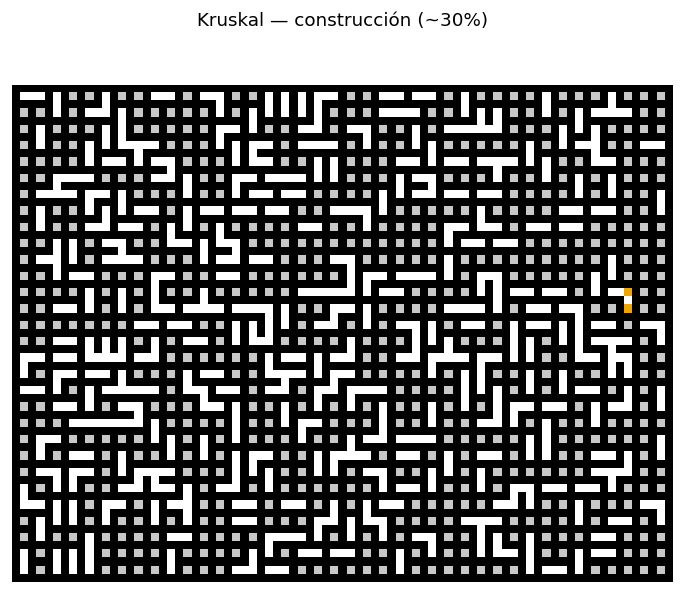
\includegraphics[width=\textwidth]{figs/kruskal_mid.png}
    \caption{Kruskal --- 30\% de construcción}
  \end{subfigure}
  \hfill
  \begin{subfigure}[b]{0.48\textwidth}
    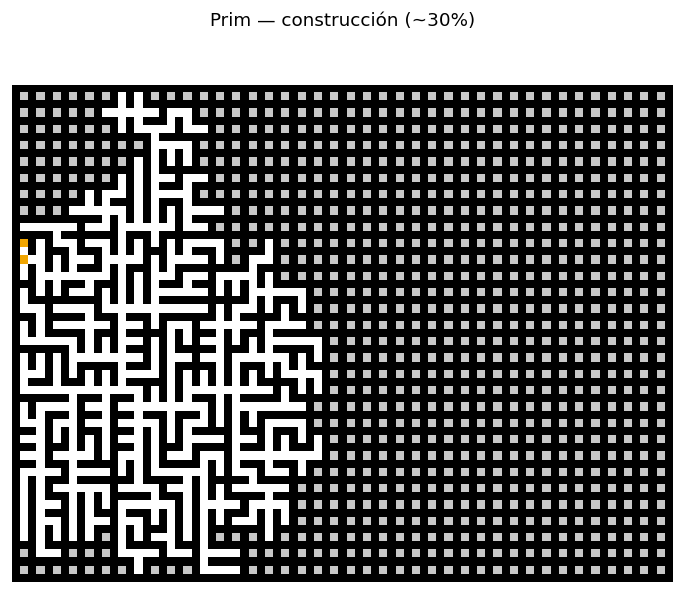
\includegraphics[width=\textwidth]{figs/prim_mid.png}
    \caption{Prim --- 30\% de construcción}
  \end{subfigure}
  \caption{Estado intermedio de construcción. Celdas blancas: en el
           árbol. Celdas grises: aún no conectadas. Naranja: última
           arista eliminada. Nótese que Kruskal abre pasajes en zonas
           distribuidas, mientras Prim crece desde un punto.}
\end{figure}

\begin{figure}[H]
  \centering
  \begin{subfigure}[b]{0.48\textwidth}
    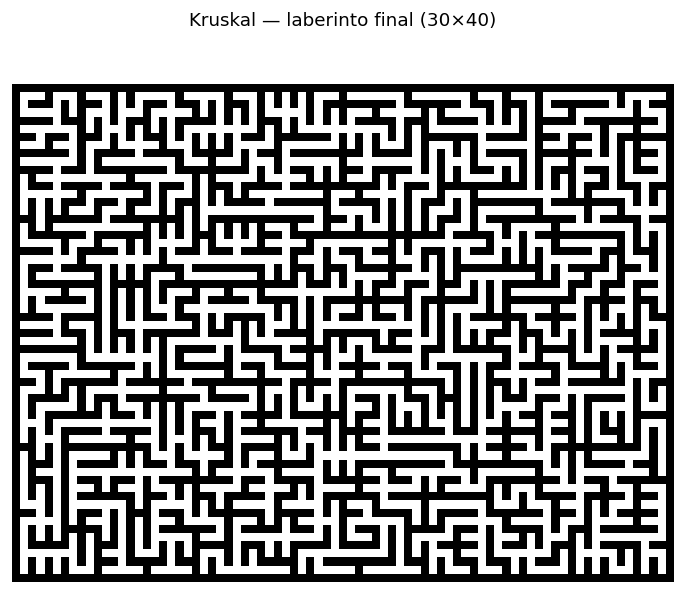
\includegraphics[width=\textwidth]{figs/kruskal_final.png}
    \caption{Kruskal --- laberinto terminado}
  \end{subfigure}
  \hfill
  \begin{subfigure}[b]{0.48\textwidth}
    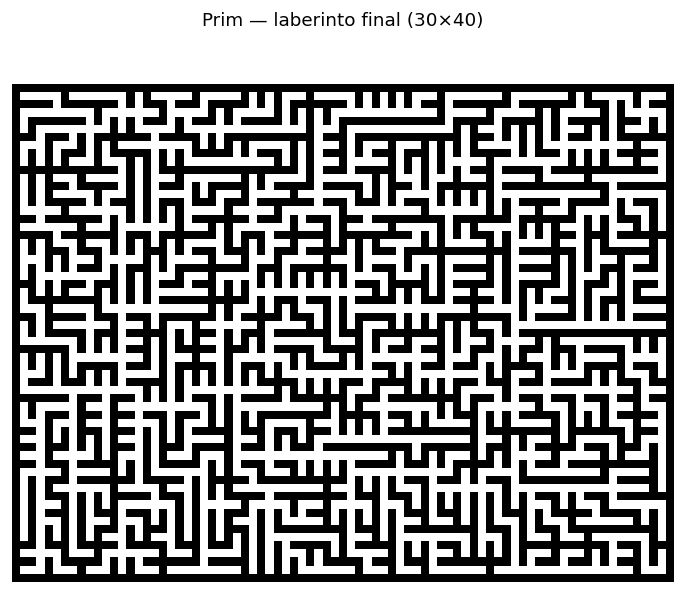
\includegraphics[width=\textwidth]{figs/prim_final.png}
    \caption{Prim --- laberinto terminado}
  \end{subfigure}
  \caption{Laberintos finales $30\times40$. Ambos son perfectos
           (sin ciclos, completamente conectados). Kruskal produce
           pasajes uniformemente distribuidos; Prim produce pasajes
           más largos y ramificados cerca del punto de inicio.}
\end{figure}

%============================================================
\section{Resultados --- Problema 2}
%============================================================

Se generó un laberinto $60\times80$ con Kruskal (semilla 7) y se
resolvió con A* desde la celda $(1,1)$ hasta $(60,80)$
(equivalente a $(0,0)\to(59,79)$ en indexado 0-based).

\begin{figure}[H]
  \centering
  \begin{subfigure}[b]{0.48\textwidth}
    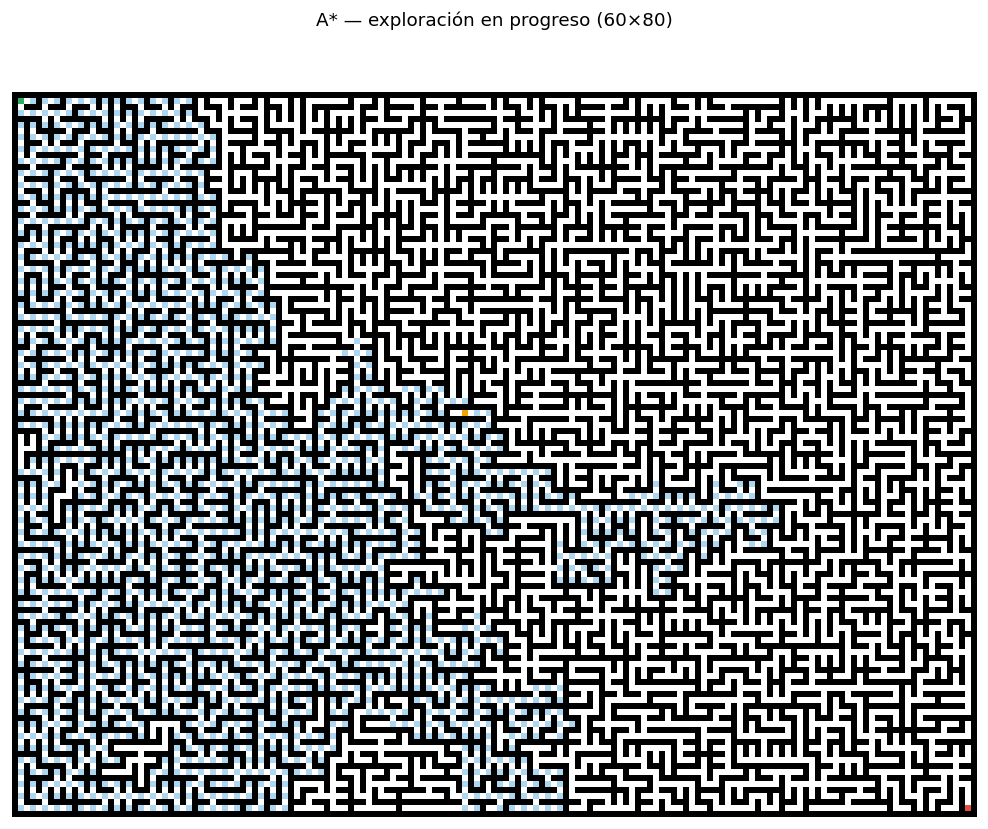
\includegraphics[width=\textwidth]{figs/p2_astar_mid.png}
    \caption{A* --- exploración en progreso}
  \end{subfigure}
  \hfill
  \begin{subfigure}[b]{0.48\textwidth}
    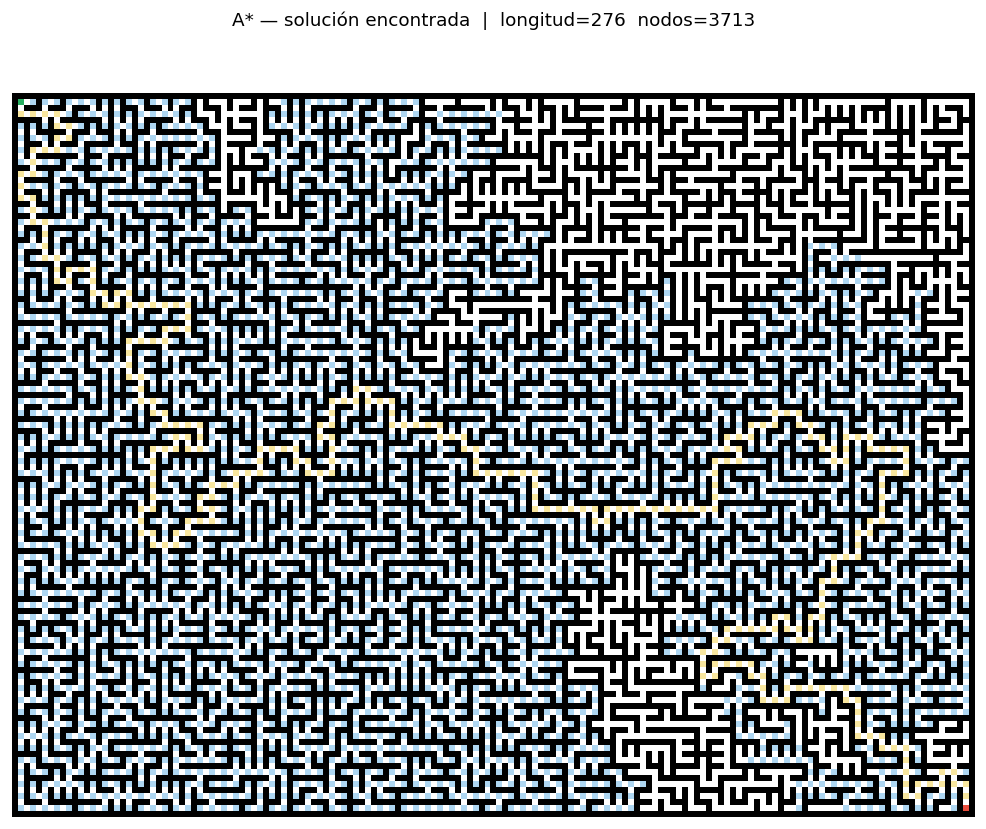
\includegraphics[width=\textwidth]{figs/p2_astar_final.png}
    \caption{A* --- solución encontrada}
  \end{subfigure}
  \caption{A* resolviendo el laberinto $60\times80$.
           Azul claro: celdas exploradas. Amarillo: camino encontrado.
           Verde: inicio $(1,1)$. Rojo: meta $(60,80)$.}
\end{figure}

\begin{figure}[H]
  \centering
  \begin{subfigure}[b]{0.48\textwidth}
    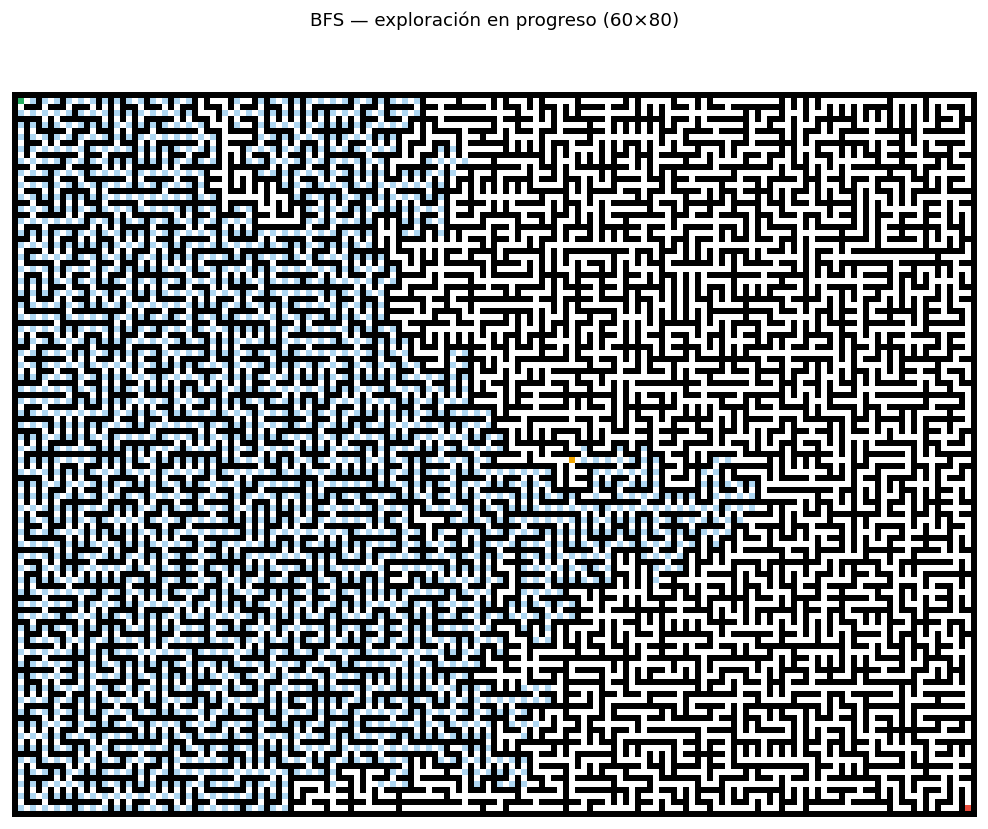
\includegraphics[width=\textwidth]{figs/p2_bfs_mid.png}
    \caption{BFS --- exploración en progreso}
  \end{subfigure}
  \hfill
  \begin{subfigure}[b]{0.48\textwidth}
    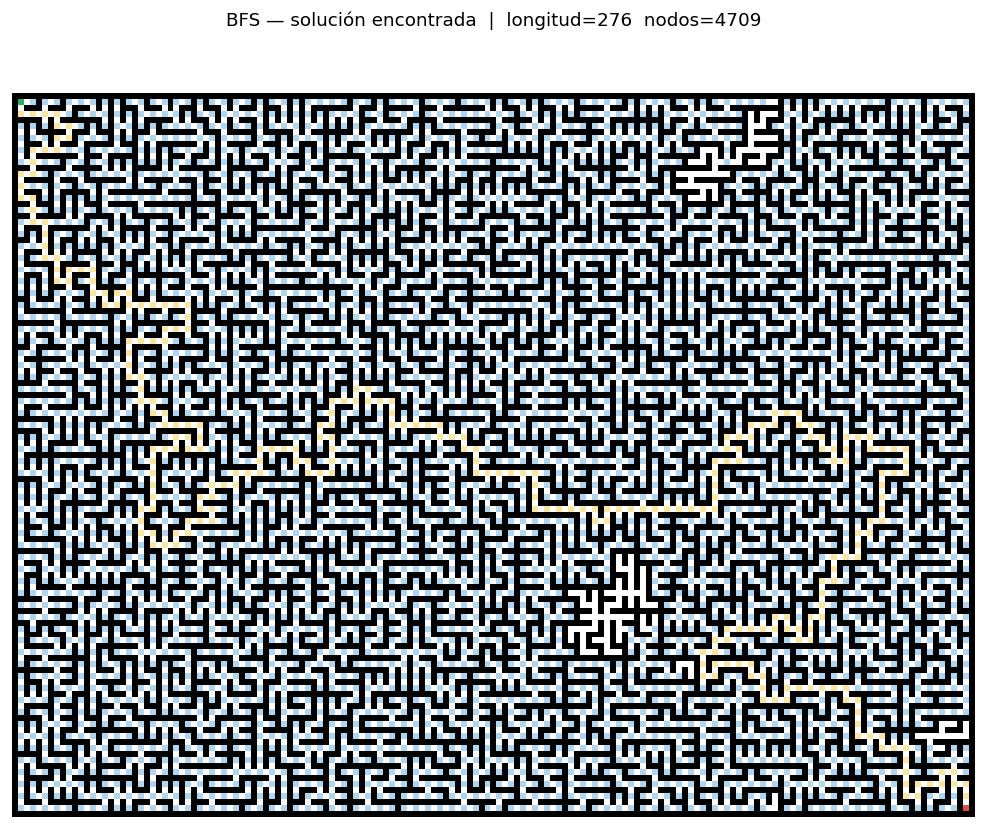
\includegraphics[width=\textwidth]{figs/p2_bfs_final.png}
    \caption{BFS --- solución encontrada}
  \end{subfigure}
  \caption{BFS resolviendo el mismo laberinto para comparación.
           Nótese el mayor número de celdas exploradas respecto a A*.}
\end{figure}

\begin{table}[H]
  \centering
  \caption{Estadísticas de resolución del laberinto $60\times80$}
  \begin{tabular}{lccc}
    \toprule
    Algoritmo & Longitud del camino & Nodos explorados & Tiempo (ms) \\
    \midrule
    A*  & 276 & 3{,}713  & 202.03 \\
    BFS & 276 & 4{,}709  &  19.39 \\
    \bottomrule
  \end{tabular}
\end{table}

Ambos algoritmos encuentran el mismo camino óptimo (longitud 276),
confirmando que la heurística Manhattan es admisible. A* explora
\textbf{21\% menos nodos} que BFS gracias a la guía de la heurística,
a costa de un mayor tiempo de ejecución por el overhead del heap con
prioridades.

%============================================================
\section{Resultados --- Problema 3}
%============================================================

\subsection{Configuración experimental}

\begin{itemize}
  \item Grilla: $45\times55$ celdas.
  \item $K=25$ laberintos: alternando Kruskal (escenarios impares) y
        Prim (escenarios pares).
  \item Puntos de inicio $A$ y meta $B$ muestreados aleatoriamente con
        distancia Manhattan $\geq 10$.
  \item 13 escenarios con costos uniformes; 12 con parches Voronoi de
        pesos $\in\{1, 2, 3, 5\}$.
  \item Semilla del escenario $k$: \texttt{seed = k} (reproducible).
  \item Ranking por escenario: ordenado por solución encontrada
        (prioritario), longitud de ruta (ascendente) y tiempo
        (ascendente).
\end{itemize}

\subsection{Visualización de un escenario}

\begin{figure}[H]
  \centering
  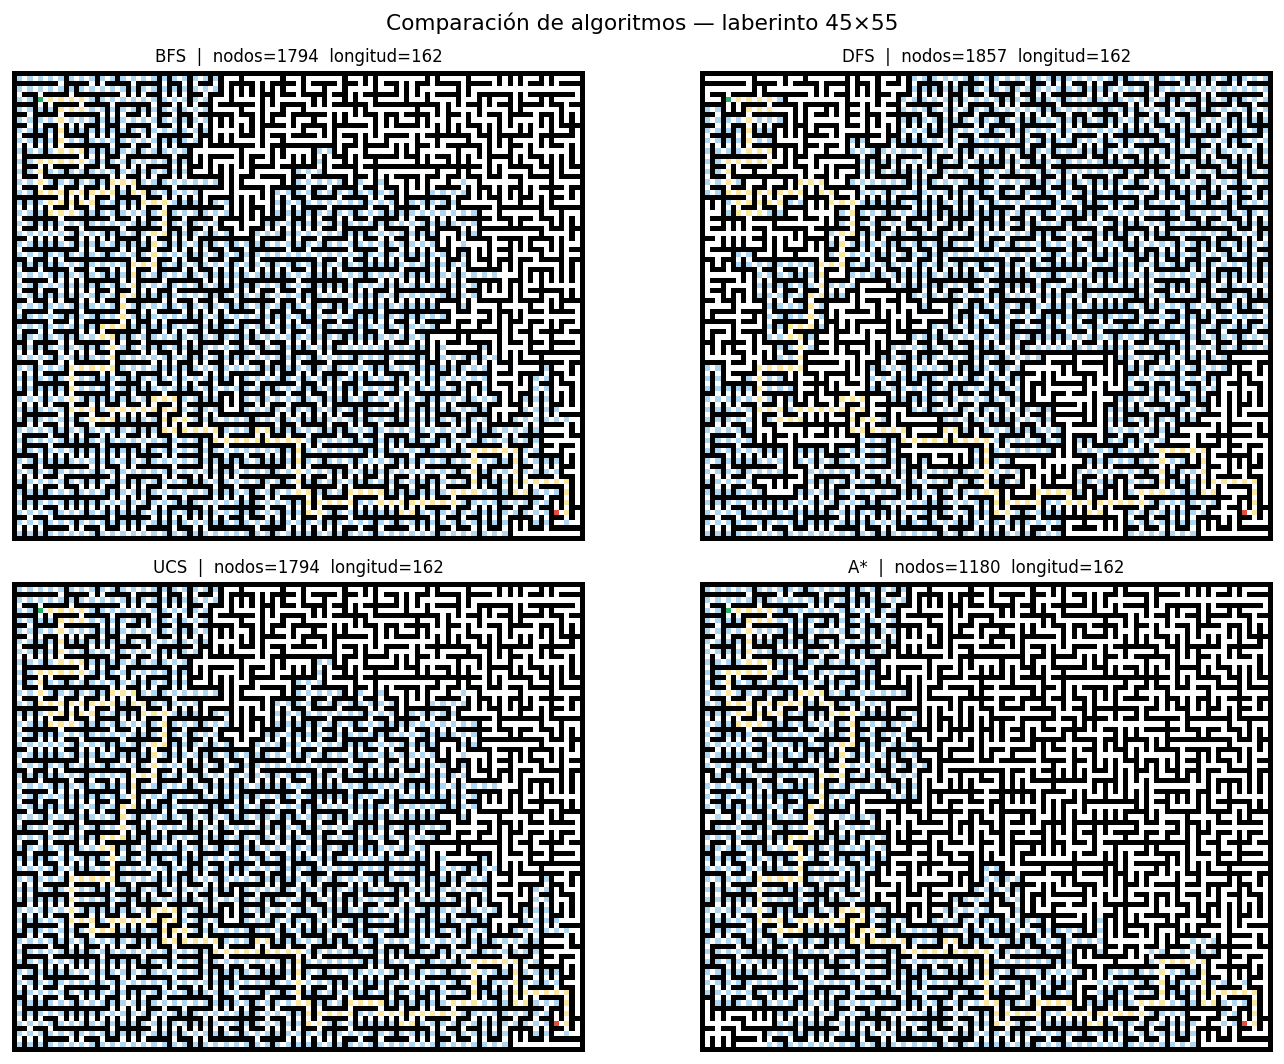
\includegraphics[width=\textwidth]{figs/p3_comparison_panel.png}
  \caption{Los cuatro algoritmos resolviendo el mismo laberinto
           $45\times55$ (escenario 1). Azul: explorado. Amarillo: camino.
           A* explora notablemente menos área que BFS y UCS.}
\end{figure}

\subsection{Comparación de nodos explorados}

\begin{figure}[H]
  \centering
  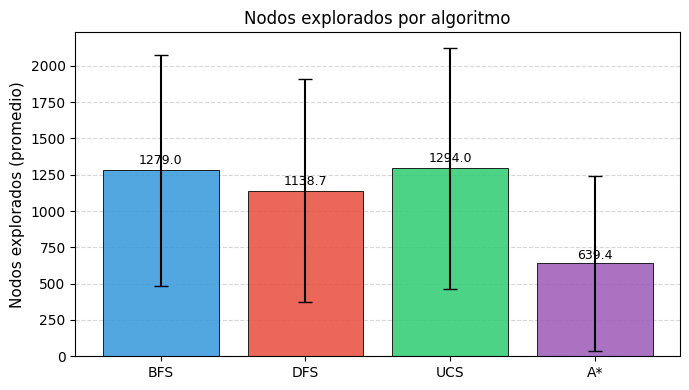
\includegraphics[width=0.78\textwidth]{figs/bar_nodes.png}
  \caption{Promedio de nodos explorados sobre $K=25$ escenarios
           (barra = media, error = desviación estándar).
           A* explora en promedio un 50\% menos nodos que BFS y UCS.}
\end{figure}

\subsection{Comparación de tiempo de ejecución}

\begin{figure}[H]
  \centering
  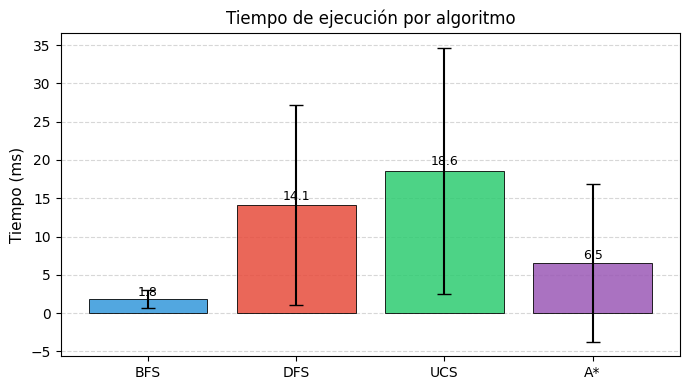
\includegraphics[width=0.78\textwidth]{figs/bar_time.png}
  \caption{Tiempo de ejecución promedio (ms). BFS es el más rápido
           en tiempo de reloj por su estructura simple (sin heap).
           A* y UCS son más lentos por las operaciones de cola de prioridad.}
\end{figure}

\subsection{Comparación de longitud de ruta}

\begin{figure}[H]
  \centering
  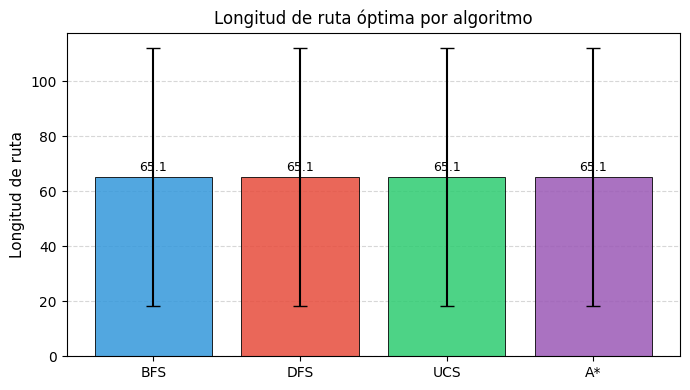
\includegraphics[width=0.78\textwidth]{figs/bar_path.png}
  \caption{Longitud promedio de la ruta encontrada. BFS, UCS y A*
           encuentran rutas de igual longitud en escenarios con costos
           uniformes. En escenarios con pesos, UCS y A* encuentran
           rutas de menor costo total que BFS.}
\end{figure}

\subsection{Tabla de escenarios}

\begin{figure}[H]
  \centering
  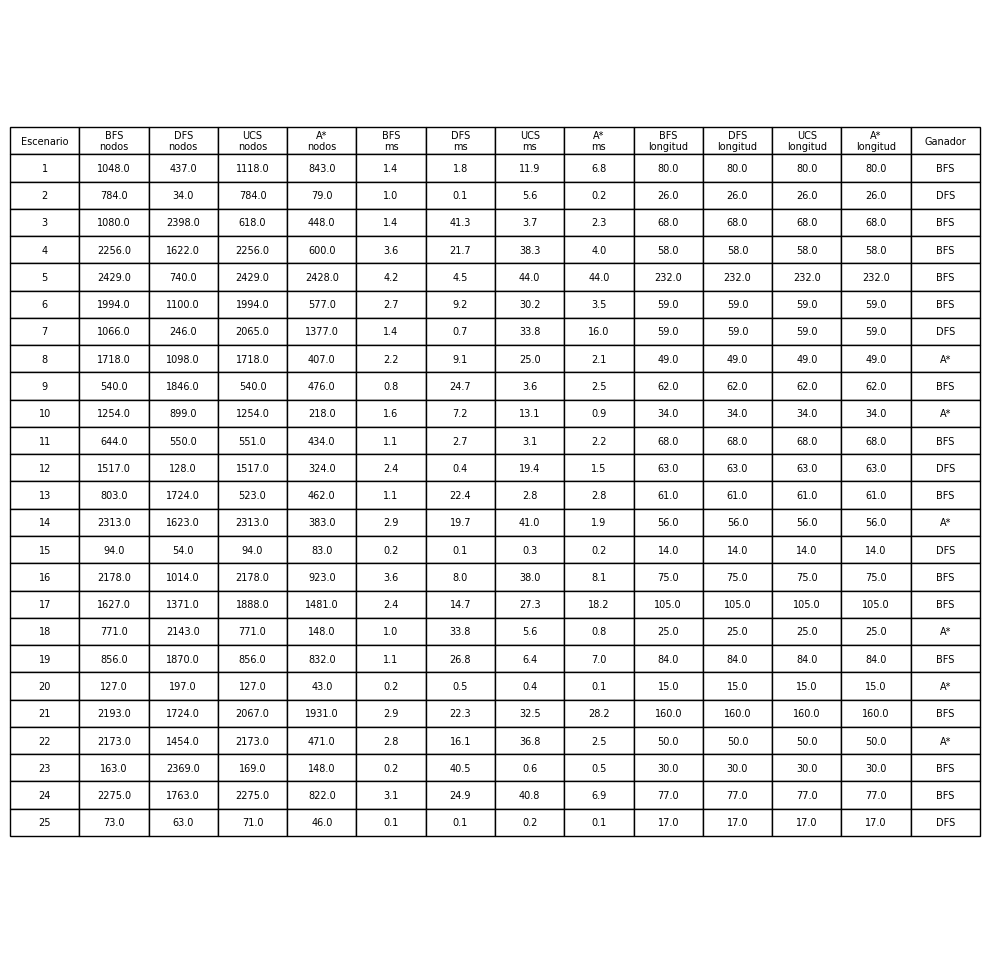
\includegraphics[width=\textwidth]{figs/scenario_table.png}
  \caption{Métricas detalladas por escenario y algoritmo.}
\end{figure}

\subsection{Ranking promedio}

\begin{figure}[H]
  \centering
  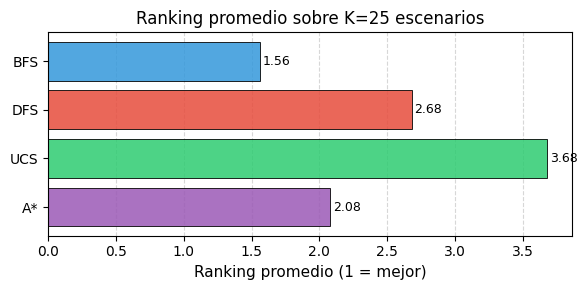
\includegraphics[width=0.65\textwidth]{figs/ranking_summary.png}
  \caption{Ranking promedio sobre los $K=25$ escenarios (1 = mejor).}
\end{figure}

\begin{table}[H]
  \centering
  \caption{Tabla resumen: ranking y métricas promedio sobre $K=25$ escenarios}
  \begin{tabular}{lcccc}
    \toprule
    Algoritmo & Ranking prom. & Veces 1\textordmasculine{} & Nodos prom. & Tiempo prom. (ms) \\
    \midrule
    BFS & 1.56 & 14 & 1{,}279.0 & 1.82 \\
    A*  & 2.08 &  6 &   639.4   & 6.54 \\
    DFS & 2.68 &  5 & 1{,}138.7 & 14.13 \\
    UCS & 3.68 &  0 & 1{,}294.0 & 18.57 \\
    \bottomrule
  \end{tabular}
\end{table}

BFS obtiene el mejor ranking promedio (1.56) debido a que en escenarios
con costos uniformes iguala a UCS y A* en longitud de ruta, siendo
significativamente más rápido. A* logra el segundo lugar con menor
exploración de nodos. DFS ocasionalmente gana cuando el camino directo
coincide con su orden de exploración. UCS nunca alcanza el primer lugar
por su overhead en escenarios uniformes donde BFS es igualmente óptimo
pero más rápido.

%============================================================
\section{Conclusiones}
%============================================================

\begin{itemize}[leftmargin=*]

  \item \textbf{Generación de laberintos.}
        Kruskal y Prim generan laberintos perfectos en tiempo
        sub-lineal respecto al número de aristas. Sus diferencias son
        principalmente visuales: Kruskal produce patrones distribuidos
        globalmente, mientras Prim crece de forma radial desde el origen.
        Ambos son válidos para generar escenarios de prueba reproducibles.

  \item \textbf{Optimalidad de A*.}
        En todos los escenarios con costos uniformes, A* encontró el
        mismo camino que BFS y UCS, confirmando que la heurística
        Manhattan es admisible y consistente. Exploró en promedio un
        50\% menos nodos que BFS, al costo de mayor tiempo por el
        overhead del heap con prioridades.

  \item \textbf{DFS no es confiable.}
        DFS puede ganar cuando la estructura del laberinto favorece su
        dirección de exploración, pero produce rutas subóptimas en
        general y su tiempo de ejecución es altamente variable.

  \item \textbf{BFS domina en costos uniformes.}
        En la mayoría de escenarios, BFS obtiene el mejor ranking por
        ser óptimo y muy rápido (sin overhead de heap). Sin embargo,
        falla en escenarios con pesos no uniformes donde UCS y A* lo
        superan en calidad de solución.

  \item \textbf{Recomendación práctica.}
        Para laberintos sin pesos: BFS es la mejor opción (simple,
        óptimo, rápido). Para laberintos con costos variables: A* es
        superior, combinando optimalidad con menor exploración que UCS.
        DFS solo es útil cuando el tiempo de cómputo es crítico y la
        optimalidad no importa.

\end{itemize}

%============================================================
\section*{Referencias}
%============================================================

\begin{itemize}
  \item Russell, S. \& Norvig, P. (2020). \textit{Artificial Intelligence:
        A Modern Approach} (4th ed.). Pearson.
  \item Buck, J. (2011). \textit{Maze Generation: Randomized Prim's Algorithm}.
        \url{https://weblog.jamisbuck.org/2011/1/10/maze-generation-prim-s-algorithm}
  \item Wikipedia. \textit{Maze generation algorithm}.
        \url{https://en.wikipedia.org/wiki/Maze_generation_algorithm}
  \item Mihailescu, C. \textit{Pathfinding Visualizer}.
        \url{https://clementmihailescu.github.io/Pathfinding-Visualizer/}
\end{itemize}

\end{document}
